\documentclass[english]{tudscrreprt}
\usepackage[T1]{fontenc}
%\usepackage[ngerman=ngerman-x-latest]{hyphsubst}
\usepackage{babel}
\usepackage{isodate}
\usepackage{tudscrsupervisor}
\usepackage{enumitem}\setlist{noitemsep}
\usepackage{siunitx}
\usepackage{tabto}

\begin{document}
\faculty{Faculty of Electrical and Computer Engineering}
\institute{Institute of Electrical Power Engineering}\chair{Chair of Electromagnetic Theory and Compatibility}
\title{%
Conducted Immunity (IEC~61000-4-6)
}\date{\today}
\contactperson{%
Prof. Hans Georg Krauthäuser\emailaddress{tetemv@tu-dresden.de}
\office{Görges-Bau, Room 223}\telephone{+49 351 463-33357}
%\and%
%Mac Moneysac\emailaddress{mac.moneysac@tu-dresden.de}
%\office{Dingens-Bau, Zimmer~15}\telephone{+49 351 463-54321}
}
\noticeform[headline=Laboratory Description,pagestyle=empty]{%
  \renewcommand{\focusname}{Parameter}
  \renewcommand{\contactpersonname}{Contact Person}
The objective of IEC~61000-4-6 is to establish a common reference for evaluating the functional immunity of electrical and electronic equipment when subjected to conducted disturbances induced by RF fields. Typical RF transmitters (sources of emissions) are:
\begin{itemize}
\item Transmitting radio systems (e.g. radio, television, mobile phones, wireless phones) cause fields that induce disturbances in lines.
\item Low-frequency interference currents of power electronics (e.g. power converters or motor drivers).
\end{itemize}
​
It is assumed that the disturbance of the electromagnetic field may act on the whole length of cables connected to installed equipment. The dimensions of the disturbed equipment are assumed to be small compared to the wavelengths involved. The in-going and out-going cables and wires: e.g. mains, communication lines, and interface cables, behave as passive receiving antenna networks (they can be several wavelengths long). Between those cable networks, the susceptible equipment is exposed to currents flowing through the equipment. 
  \begin{center}
  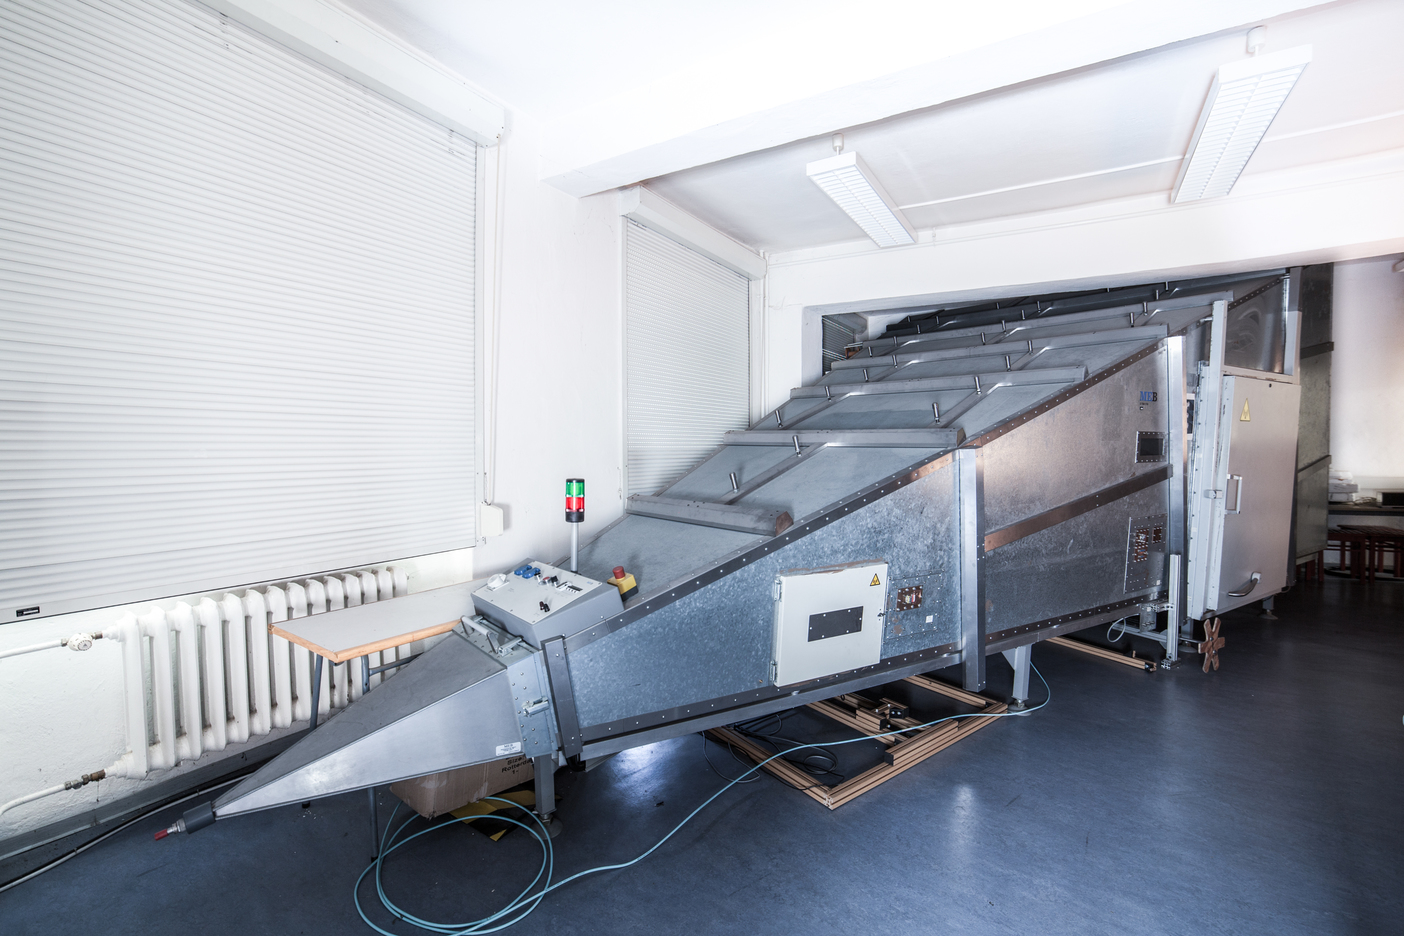
\includegraphics[width=.65\linewidth]{gtem_cell_aussen_hell_klein}
\renewcommand*{\figureformat}{Photo}
\captionof{figure}{Example Setup.}
\end{center}
}{%
\item Frequency range:\tabto{.3\linewidth} \qty{150}{\kilo\hertz} -- \qty{250}{\mega\hertz} (\qty{1}{GHz})
\item Available Power: \tabto{.3\linewidth} $\le$ \qty{80}{\watt}
\item Test Levels: \tabto{.3\linewidth} 1, 2, 3, X\\
  \tabto{.3\linewidth} \qty{30}{V} (CDN), \qty{20}{V} (EM Clamp), \qty{10}{V} (Current Injection)
\item Networks (CDN): \tabto{.3\linewidth} M1, M3, EM clamp
\item Main Standards:
  \begin{itemize}
  \item IEC~61000-4-6, EN~61000-4-6, DIN~EN~61000-4-6
    \end{itemize}
}
\end{document}